\begin{figure}[htb]
  \centering
  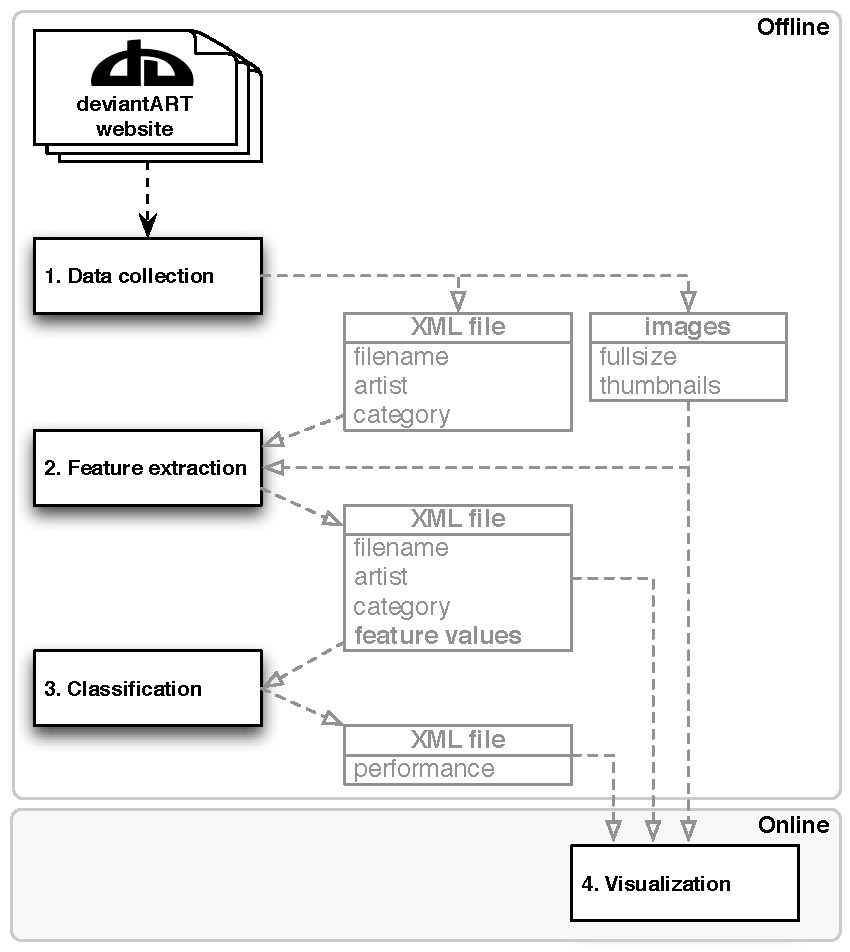
\includegraphics[width=1\linewidth]{img/components.pdf}
  \caption{Interaction between the four components of the toolkit.}
  \label{fig:components}
\end{figure}

Our toolkit consists out of four replacable components.
Each component writes its output (e.g. image information and features) to a XML file.
The first three components are all executed \textit{offline} (pre-calculated), while the visualization component allows \textit{online} interaction with the images, features and classification results.
Fig.~\ref{fig:components} provides an overview of all components and the data flow between those components.

% toolboxes used
\subsection{Data collection}
The data collection component deals with downloading information and galleries from the deviantART website and it can easily be replaced to allow the toolkit to be flexible and be able to deal with different art community webpages.

DeviantArt does not provide a web API to download images and therefor the backend links of the galleries to the RSS XML files were followed to access
the image data. For each image general information such as category, deviantART link and filename are stored, and the full image and 
thumbnails are downloaded.

For the network information collection the friends pages 
of the users are parsed. No RSS XML files are provided by deviantART for this
information, instead the HTML pages were parsed.


\subsection{Feature extraction}
All the toolkit and the library used in this research field, as the code written to extract the features, are written in Matlab programming language.
Part of the statistical feature calculations were done using openCV\footnote{http://opencv.willowgarage.com/wiki/Welcome} \ref{openCV} code to speed up the feature extraction. openCV was used for color-space transformations, edge,corner and face-detection.

As it has already been explained in section \ref{proposed-cognitive}, the research focused also on the extraction of some cognitive-inspired features. First a saliency map and 4 conspicuity maps (color, intensity, orientation and skin) are computed and then the features are extracted. To create the maps it has been used the Itti's model \cite{Itti_model} due to its low computentional time and the existense of a free toolkit \footnote{http://www.saliencytoolbox.net/} made by Dirk Walther. 

The XML-processing was done using an open-source XML-toolkit~\footnote{\url{http://www.mathworks.com/matlabcentral/fileexchange/4278}}~\cite{geusebroek2005six}.

\begin{table}[htb]
    \centering
    \begin{tabular}	{ | l | } 
		\hline
		Feature \\
		\hline
		Average: Red, Blue, Green, Hue, Saturation, Intensity \\
		Median: Red, Blue, Green, Hue, Saturation, Intensity \\
		Variance: Intensity \\
		Edge detection \\
		Corner detection \\
		Face detection \\
		stdev: saliency map, conspicuity maps \\
		Entropy: Intensity, saliency map, conspicuity maps \\
		\hline
    \end{tabular}
    \caption{Overview of features}
    \label{tab:featurelist}
\end{table}

\subsection{Classification}
The classification part of this toolkit was implemented in Matlab.
For the kNN, naive bayes, nearest mean classifiers and the feature selection PRTools\footnote{http://prtools.org/} \cite{Duin00prtoolsversion} was used.
This toolkit provides functions to create a dataset format that can be used for all three of the classifiers.
Furthermore the dataset can be managed using this toolkit.

The SVM classifier was implemented using libSVM\footnote{\url{http://www.csie.ntu.edu.tw/~cjlin/libsvm/}} \cite{chang2001libsvm} for Matlab.
LibSVM contains a C implementation of the SVM classifier which results into considerably higher processing speed compared to the Matlab environment.

%\subsection{Classification}
%An important aspect of analyzing images is to determine what makes them distinct.
%In this tookit, classification is used to compare image sets and extract the image features that best separates them.
%This knowledge can be used to describe the art style of an artist or even determine if there is an artist that uses an unique style.
%Also classification can be extended to other category level to determine what the image features of a category are.
%
%\subsubsection{Pre-processing}
%Before classifiers can be used to find image features, several pre-processing steps are required on the dataset.
%
%Naturally, functions that read in XML files containing the feature values, convert it to a dataset and splitting it into a train and test set are incorporated.
%Also Min/Max normalization can be used on the dataset.
%Normalization is important because the features that were extracted all uses different ranges of values, by scaling these values to the same range(e.g. [-0.5,0.5]), classifiers are more effective in their task to find image features that separates a class from the other classes.
%
%Furthermore filtering on classes and features can be performed on the dataset, this is to provide flexibility in a way that the user can do classification on just a few interesting classes or features instead of everything that is inside the dataset.
%
%\subsubsection{Classifiers}
%The classification part of the toolkit is implemented using the Matlab environment. In total there are four different classifiers that be called upon.
%
%\begin{itemize}
%	\item \textbf{k-Nearest Neighbour}: It classifies images based on the closest training examples.
%	This classifier uses a parameter $k$ that can be optimized. 
%	The parameter indicates how many of the training examples the classifier should compare the new image with before it can classify to what class an image belongs to.
%	\item \textbf{Naive Bayes}: It calculates the probability of a new image belonging to a class.
%	This classifier takes every feature seperately and divide it into $N$ bins, it will then count the number of training examples for every class in all the bins and uses this to compute the posterior probability.
%	$N$ is used here as a parameter that can be optimized.
%	\item \textbf{Nearest Mean}: It calculates the mean value of a class and classifies new images based on how close it lays to the mean of a class.
%	\item \textbf{Support Vector Machine}: It creates a model based on a set of training examples which belongs to two classes.
%	The SVM tries to divide the training examples by a clear gap and then predicts the class of a new example based on which side of the gap it lays.
%\end{itemize}
%
%The classifiers were implemented using PRTools \cite{Duin00prtoolsversion} and libSVM \cite{chang2001libsvm}, which are existing implementations of the classifiers.
%
%\subsubsection{Feature Selection}
%Whenever a person wants to find the image features that best separates two classes, that person wants to have a small list containing image features that does that.
%Therefore a feature selection algorithm is needed to make sure that the classifier will only choose a few features(e.g. 1,2,3) instead of a whole list of features which does not say anything interesting.
%
%Features were selected by using the \textit{Sequential forward feature selection} \cite{pudil1994floating}.
%It selects features by first choosing the most informative feature and then iteratively add the next most informative feature to it.
%Selecting the most informative feature is done using the inter-intra criterion \cite{pekalska2005pairwise}.
%This criterion is computed based on the average dispersion of a class around its mean and the distance of mean to the overall average value of the dataset.
%Therefore the features that are selected are the features that clusters the class while eliminating the overlap between that cluster and the other classes.
%
%\subsubsection{Evaluation Measures}
%For classification the \textit{precision} and \textit{recall} are used as evaluation measures for how well a classifier performs.
%The precision is computed by measuring how many percent of the examples were correctly classified as positive as opposed to how many of all examples were classified as positive.
%The recall is computed by measuring how many percent of the positive examples were indeed classified as positive.
%The total performance score of the classifier can be calculated using the $F_1-measure$.
%The $F_1$-measure is the weighted average of the precision and recall scores where they are both weighted as equally importance.
%For our toolkit a high $F_1$-measure means that the features that were used to classify an artist are reliable features to separate the artist from the other artists in the set.
%
%\subsubsection{Parameter Optimization}
%Another important aspect of classification is to do parameter optimization. 
%Optimization of parameters will lead to better classification results because the classifier is more fine tuned to the type of task that lies ahead. 
%The way the optimization is presented in this toolkit is by cross-validation on the train set.
%For every parameter in the classifier cross-validation is performed on the trainset to compute the F-measure score.
%The average F-measure score of every fold is used as an evaluation measure to indicate how well the classifier performs.

% which classifiers
% how they work
% how they operate in the system


\subsection{Visualization}
The final component of the toolkit is the visualization application.
This visualization is used to present the information that has been gathered by the other components of the toolkit.
The collected images are used together with the extracted image features (Fig.~\ref{fig:components}) to visualize the dataset.
This provides an effective way to find patterns in the dataset, analyze classification results and filter information.
The visualization application combines three different visualization techniques into one application.
Each visualization technique offers a different look on the dataset.

There are multiple data visualization applications and toolkits~\footnote{Wikiviz \url{http://www.wikiviz.org/wiki/Tools}} that are able to create visualizations out of the box.
But these applications and toolkits offer only generic displays and interactions, which do not capture the dataset in its full potential.
This disadvantage convinced us to create our own application.
The visualization application is written in the Java programming language.
The open source Processing API \footnote{\url{http://www.processing.org}} is used to draw the visualizations of the application.
The Processing API contains classes and functions that simplify drawing, animations and interactions in Java.
Processing was an obvious choice, because it has the right combination of cost, ease of use and speed~\cite{fry08}.

\begin{figure}[htb]
  \centering
  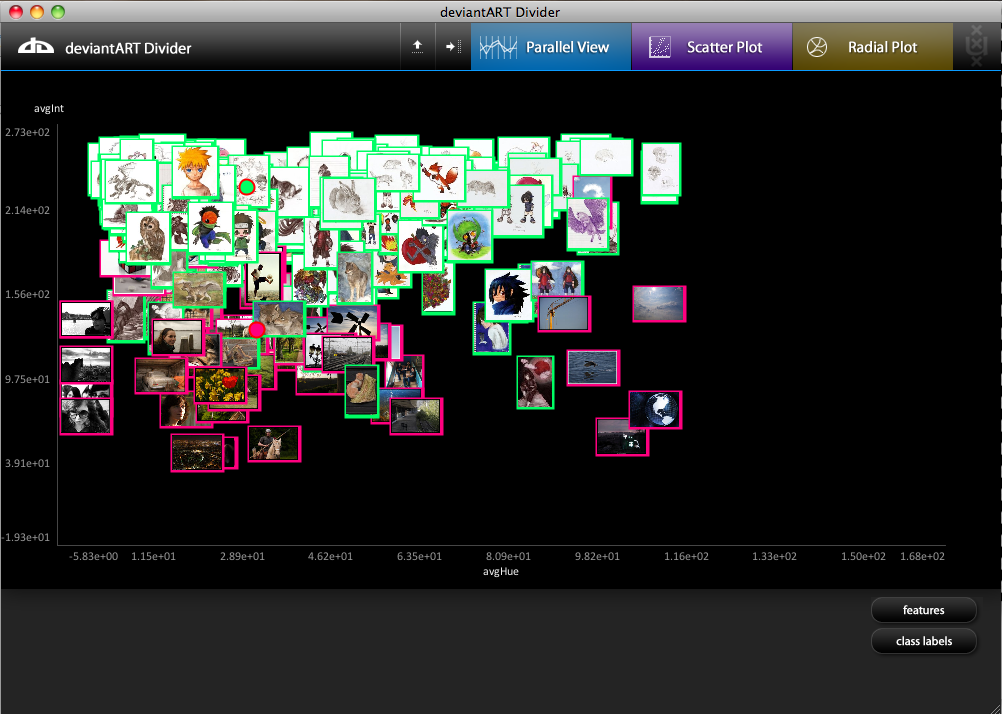
\includegraphics[width=1\linewidth]{img/visualization_scatter.png}
  \caption{The visualization application displaying a scatter plot of 2 artists.}
  \label{fig:visualization_scatter}
\end{figure}

Fig.~\ref{fig:visualization_scatter} shows the \textit{scatter plot} visualization technique.
The scatter plot displays values for two variables, which are image features that has been computed by the \textit{feature extraction} component.
The data is displayed as a collection of thumbnail images.
Each thumbnail has the value of one feature determining the position on the horizontal axis and the value of the other feature determining the position on the vertical axis.
The border around each image represents the class (artists or category) to which an image belongs.
For example, the images with a green border belong to the artist \textit{Kitsunebaka91} and the images with a red pink border belong to the artist \textit{Woekan}.
The user has full control over which classes are displayed in the visualization.
The users can also control which two features are used as variables on the horizontal and vertical axis of the scatter plot.
A single image or all the images belonging to one class can be highlighted, making it more easy to recognize patterns.
The full version of a miniature image can be displayed to inspect it in more detail.

\begin{figure}[htb]
  \centering
  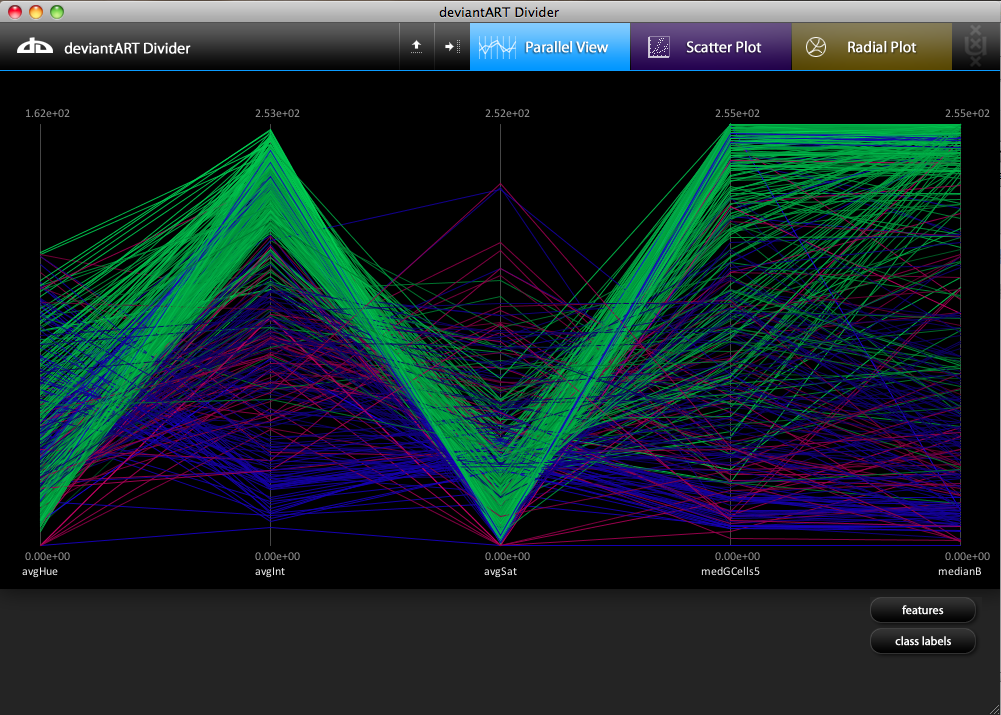
\includegraphics[width=1\linewidth]{img/visualization_parallel.png}
  \caption{The visualization application displaying a parallel coordinates plot of 3 artists and 5 features.}
  \label{fig:visualization_parallel}
\end{figure}

The scatter plot is limited to displaying only two features at the same time.
Fig.~\ref{fig:visualization_parallel} shows the \textit{parallel coordinates} visualization technique~\cite{andrienko2001constructing}, a common way of visualizing high-dimensional.
This enabled us to visualize beyond two features at the same time.
The two axes of the scatter plot are now replaced by $n$ vertical parallel lines to represent $n$ features ($n$-dimensional space).
An image is now represented as a polyline with vertices on the parallel axes.
The color of a polyline represents the class (artist, category) to which an image belongs.

\begin{figure}[htb]
  \centering
  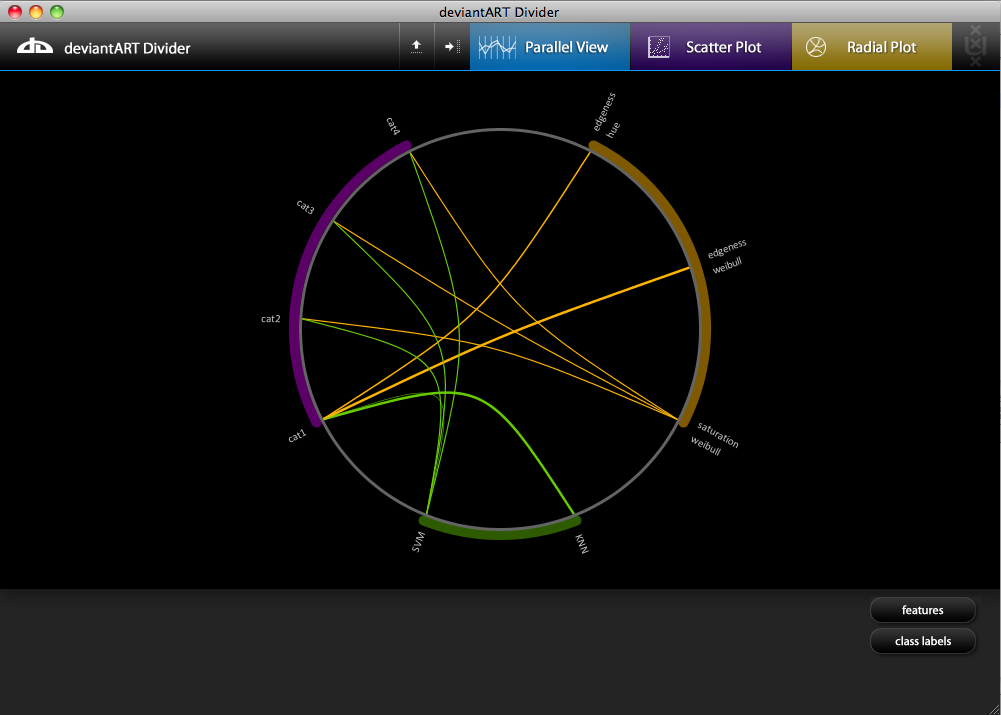
\includegraphics[width=1\linewidth]{img/visualization_radial.png}
  \caption{The visualization application displaying a radial plot that expresses the performance of the classification.}
  \label{fig:visualization_radial}
\end{figure}

Fig.~\ref{fig:visualization_radial} shows the \textit{radial plot} visualization technique.
This visualization is not used to visualize the dataset, but to display the performance of the classification, e.g., how a certain feature performs on separating an artist from the other artists.
The circle is split into three regions (variables): artists or categories (purple), features (yellow), classifiers (green).
%Each of these regions represent a variable that plays an important role in the classification of images.
%Each variables consists of a limited number of values that were used during classification.
The thickness of a line between two nodes expresses the performance of the classification when both nodes are used together, i.e., thicker lines means higher performance.
For example, a thick line between artist X and feature Y, means that feature Y is a good feature to separate artist X from the other artists.
